\section{Data-Driven Testing}

Data-driven testing is a scripting technique that stores test inputs and
expected outcomes as data, normally in a tabular format, so that a single
driver script can execute all of the designed test cases~\cite{Fewster99}.
Usually, testing scripts that don't follow a data-driven approach, have data
attached into them. When test data needs to be updated the actual test script
must be changed as well. This might not be a big deal for the person who
originally implemented the script but it may become a problem to a test engineer
that has less programming experience.

Data represents a large part of system and test specification. By considering
how data is defined and used during testing we can increase the opportunity
of reuse as well as reduce future maintenance costs for subsequent releases of
the system being developed. That's what make data-driven testing extremely
useful since one single test script can be used to run different tests reducing
the number of the overall test scripts needed to implement all the test cases.

\begin{table}[!ht]
\centering
\begin{tabular}{lllll}
\textbf{Test Case} & \textbf{Input 1} & \textbf{Operation} & \textbf{Input 2} & \textbf{Result} \\
Addition 01 & 5 & + & 5 & 10 \\
Addition 02 & 5 & + & 10 & 15 \\
Subtraction 01 & 10 & - & 5 & 5 \\
Subtraction 02 & 10 & - & 0 & 10 \\
Multiplication 01 & 5 & * & 5 & 25 \\
Multiplication 02 & 5 & * & 0 & 0 \\
Division 01 & 10 & / & 2 & 5 \\
Division 02 & 10 & / & 10 & 0 \\
\end{tabular}
\caption{Data-driven test data with mathematical operations.}
\label{table:tab1}
\end{table}

A suitable scenario where data-driven testing can be applied is when two or more
test cases requires the same instructions but different inputs and different
expected outcomes. The refactoring would result in one single test script and a
shared input data file.

\subsection{Storing Test Data}

Data-driven testing calls for tabular data and the first instinct is to use
spreadsheet programs to edit it~\cite{Lau07}. Spreadsheet files like
comma-separated-values (CSV) are handy because they are very easy to parse but
unfortunately the data becomes inconsistent when edited by two or more different
spreadsheet programs. But the biggest problem with storing test data into any
kind of flat file is scalability~\cite{Lau07}. If for example test data is
created and edited in several workstations and used in multiple test
environments it gets hard to have the same version of the data everywhere.
Moving the data files to a central database, backed up by a web-based
interface in order to manage the test data, is a suitable solution when
scalability is a requirement. This way, the driver scripts can read test data
directly from the database instead of parsing CSV files before running the
test suite.

\subsection{Processing Test Data}

Implementing a script for parsing data-driven test data can be surprisingly
easy either using data files or databases~\cite{Lau07}. Data is processed line
by line and split into cells that represent the test inputs making the data
available to be used in the test scripts. The main drawback is that the parser
will always be limited in extensibility and it will crash if the test data
format changes.

\begin{figure}[!ht]
\centering
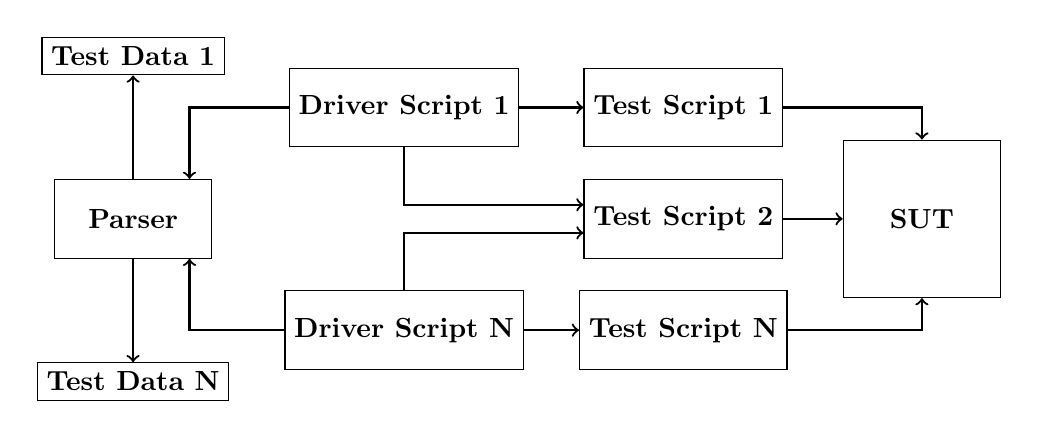
\begin{tikzpicture}
\matrix [column sep=7mm, row sep=-1mm] {
  \node (data1) [draw, shape=rectangle] {\textbf{Test Data 1}}; & & & \\
  & \node (script1) [draw, shape=rectangle,minimum width=2cm,
  minimum height=1cm] {\textbf{Driver Script 1}}; & 
  \node (tscript1) [draw, shape=rectangle,minimum width=2cm,
  minimum height=1cm] {\textbf{Test Script 1}}; \\
  \node (parser) [draw, shape=rectangle,
  minimum width=2cm, minimum height=1cm] {\textbf{Parser}}; & &
  \node (tscript2) [draw, shape=rectangle,minimum width=2cm,
  minimum height=1cm] {\textbf{Test Script 2}}; &
  \node (sut) [draw, shape=rectangle, minimum width=2cm,
  minimum height=2cm] {\textbf{SUT}}; \\
  & \node (scriptn) [draw, shape=rectangle,minimum width=2cm,
  minimum height=1cm] {\textbf{Driver Script N}}; & 
  \node (tscriptn) [draw, shape=rectangle,minimum width=2cm,
  minimum height=1cm] {\textbf{Test Script N}}; \\
  \node (datan) [draw, shape=rectangle] {\textbf{Test Data N}}; & & \\
};
\draw[->, thick] (parser) -- (data1);
\draw[->, thick] (parser) -- (datan);
\draw[->, thick] (script1) -| ([xshift=2cm,yshift=5mm]parser);
\draw[->, thick] (scriptn) -| ([xshift=2cm,yshift=-5mm]parser);
\draw[->, thick] (script1) -- (tscript1);
\draw[->, thick] (script1) |- ([yshift=5mm]tscript2);
\draw[->, thick] (scriptn) |- ([yshift=-5mm]tscript2);
\draw[->, thick] (scriptn) -- (tscriptn);
\draw[->, thick] (tscript1) -| (sut);
\draw[->, thick] (tscript2) -- (sut);
\draw[->, thick] (tscriptn) -| (sut);
\end{tikzpicture}
\caption{Data-driven approach.} \label{fig:F1}
\end{figure}

Whatever design decisions are made about the driver script, the test data must
reflect to it~\cite{Fewster99}. This means that if we change either the driver
or the format of the data, we need to make sure they are always in sync.

\subsection{Advantages of data-driven testing}

A major advantage of the data-driven testing is that the format of the
data file can be tailored to suit the testers needs~\cite{Fewster99}. The data
file can contain comments that the script will ignore but that will make the
data file much more understandable and, therefore, maintainable even by
non-technical people. The easier it is, the quicker and less error prone it
will be.

With data-driven testing we can really start to benefit from test automation~\cite{Fewster99}.
It is possible to implement many more test cases with very little extra effort
since all we have to do is specify a new set of input data and expected results
for each additional test case.\\[1mm]

\noindent Summarizing the advantages of the data-driven approach:

\begin{itemize}
\item Reduces the number of overall test scripts needed to
implement all the test cases;
\item Less amount of code is required to generate all the test cases;
\item Offers greater flexibility when it comes to maintenance and fixing of bugs;
\item The test data can be created before test implementation is ready or even
before the system to be tested is ready.
\end{itemize}

\subsection{Disadvantages of data-driven testing}

The biggest limitation of the data-driven approach is that all test cases are
similar and creating new kinds of tests requires implementing new driver scripts
that understand different test data. Thus the test data and driver scripts are
so strongly related that changing either requires changing the other. In general,
test data and driver scripts are strongly coupled and need to be always
synchronized~\cite{Fewster99}. If we look closer at the input data presented in
Table \ref{table:tab1} we can see that was designed only to accept two inputs
and in order to support operations like 10 * 5 - 5 = 45 would require major
changes on both test data and driver scripts.

The initial set-up effort of a data-driven testing framework is high~\cite{Fewster99}.
Writing the right drivers need to be done by someone with programming skills,
and not all of teams have resources to spend time on setting up testing
frameworks. Although, the benefits gained will vastly outweigh this upfront cost
when the test suit grows.

It is not appropriate for small systems where the cost of writing test cases is
not so high~\cite{Fewster99}. If a data-driven approach is used it will entail
more work, and will seem excessive. On the other hand, large and complex systems
gain far more in saved effort than you put in.\\[1mm]

\noindent Summarizing the disadvantages of the data-driven approach:
\begin{itemize}
\item Initial set-up takes of lot of effort;
\item Programming support is required;
\item It must be well managed.
\end{itemize}
